\documentclass{article}

\usepackage{geometry}
\usepackage{setspace}
\usepackage{graphicx}
%\usepackage{natbib}
\usepackage [english]{babel}
\usepackage [autostyle, english = american]{csquotes}
\MakeOuterQuote{"}

\geometry{
    top=3cm,
    bottom=3cm,
    left=3.5cm,
    right=3.5cm,
    headheight=14pt,
}

\title{A Review of the Reservoir Concept in Reservoir Computing}
\author{Neil Babson\\ \texttt{nbabson@pdx.edu}}
\date{Portland State University -  \today}

\begin{document}

\maketitle

\doublespacing

\begin{abstract}

Reservoir Computing is a computational framework in which a 
dynamical system, known as the \textit{reservoir}, casts a temporal input 
signal to a high-dimensional space, and a trainable \textit{readout layer} 
creates the output signal by extracting salient features from the reservoir.
A suitable reservoir  must possess the property of 
\textit{fading memory} in order to process inputs. The foundations of Reservoir Computing are the 
independently proposed Echo State Networks and Liquid State Machines, both of 
which use a randomly connected artificial recurrent neural network as the 
reservoir. Since the inception of the field, researchers have looked for ways 
to optimize the selection of reservoir construction parameters. Hierarchical 
reservoirs reimpose a degree of topological structure on reservoir connectivity 
by breaking the monolithic reservoir into loosely connected sub-reservoirs. The 
realization that dynamical systems besides neural networks could act as 
reservoirs has caused increasing interest in alternative reservoir substrates 
using biological, chemical, and physical dynamical systems.

\end{abstract}
% 70 words junk: g ctrl-g for word count
\section{Introduction}\label{introduction}
Reservoir Computing (RC) is a relatively new approach to machine learning in 
which  the inner dynamics of a recurrently connected system, the 
\textit{reservoir}, are harnessed to cast temporal inputs into a 
high-dimensional space, enhancing their separability.  A \textit{readout layer} 
generates the output from a linear combination of the states of reservoir 
nodes. Figure \ref{reservoir_layout} shows the components of a reservoir 
computing system. The idea of reservoirs as a new type of architecture for 
Recurrent Neural Networks (RNNs) was proposed independently in 2001, under the 
name Echo State Networks (ESNS) \cite{jaeger2001echo}, and in 2002 as Liquid 
State Machines (LSMs) \cite{maass2002real}. The recurrent connections of a RNN 
cycle information back to the internal nodes, allowing them to possess 
\textit{state}, or memory, which makes them suitable for sequential tasks such 
as speech recognition. Unlike traditional neural networks, the internal weights 
between the nodes of the reservoir used in RC are not trained.  Only the 
weights to the output layer are trained, providing a substantial reduction in 
the amount of computation required for learning. \par  A reservoir capable of 
representing the inputs in its internal dynamics can perform multiple 
computation tasks, even simultaneous tasks, by training different readout 
layers to extract the output. In both the original ESN and LSM reservoir design
nodes connect at random, but as reservoirs found a growing number of successful 
applications, researchers examined alternate construction techniques 
\cite{lukovsevicius2007overview} and showed that many types of system besides 
RNNs produce effective reservoirs \cite{tanaka2018recent}.\par
   
    This paper provides a  brief review of the main lines of investigation into 
    reservoir construction. In Section \ref{esn} and Section \ref{lsm} we 
    examine the original ESN and LSM designs. Section \ref{design} presents 
    research into modifications to RNN reservoir design, while Section 
    \ref{alternative} examines non-RNN based
    reservoir research.  Conclusions and reflection on the current state of 
    reservoir research is in Section \ref{conclusion}.  \begin{figure}[ht]
        \centering
            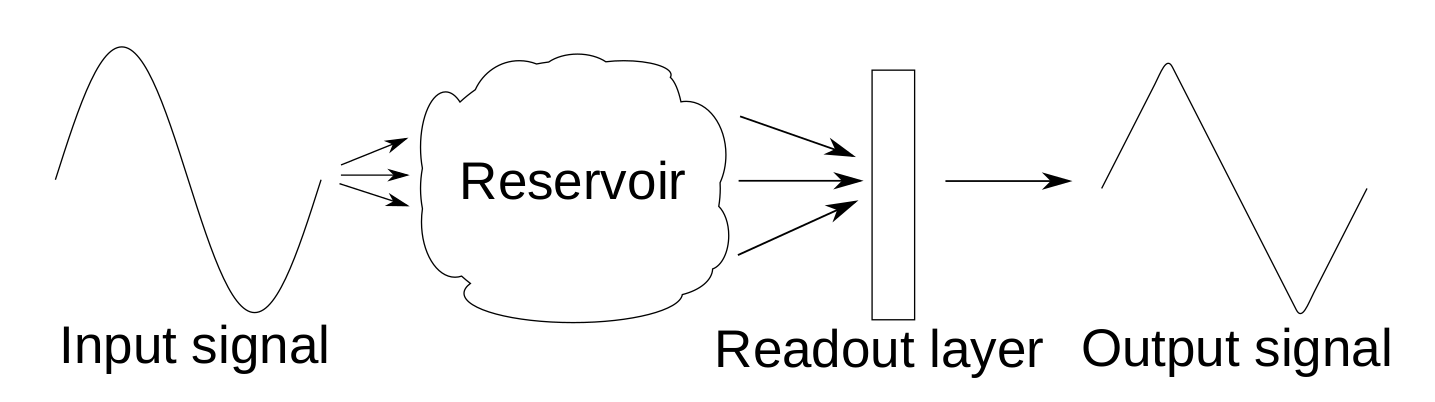
\includegraphics[width=0.5\textwidth]{reservoir_layout.png}
    \caption{Main components of a reservoir computing system. 
        \cite{bye2016investigation}}
            \label{reservoir_layout}
            \end{figure}
            \section{Foundations}\label{foundations}
            \subsection{Echo State Networks}\label{esn}
    H.  Jaeger was motivated to investigate Echo State Networks (ESNs) by the 
    difficulties encountered in training traditional RNNs, caused by factors 
    such as vanishing and exploding gradients, slow convergence, and local 
    minima  \cite{jaeger2001echo}. In order for an ESN to perform useful 
    computation, it must possess the \textit{echo-state property}, 
    characterized by the term \textit{fading memory}. The system has the 
    ability to remember (or echo) inputs, but also forgets them over time. In 
    Jaeger's words, "in order to know the current network output with a given 
    precision, we only have to know the most recent inputs with a similar 
    precision" \cite{jaeger2001echo}. The \textit{echo-state property} 
    guarantees that the input driving the ESN will "wash out" the influence of 
    the random initial condition of the reservoir, causing it to react 
    predictably to inputs \cite{jaeger2001echo}.\par An ESN consists of 
    internal discrete-time sigmoid-function nodes, as well as input and output 
    nodes. The only constraints on the network topology are that no nodes have 
    directed connections to input nodes, and that internal recurrent pathways 
    exist. The input layer maps the input signal onto the reservoir, which is 
    then "tapped" by the output layer whose weights are the only part of the 
    system that is trained. Figure \ref{esn_jpg}, taken from Jaeger's 2001 
    paper,  depicts the network architecture.\par To create ESNs with effective 
    reservoirs, the internal nodes are connected randomly but sparsely.  
    Scaling the internal connection-weight matrix so that its spectral radius 
    (the largest absolute value of its eigenvalues) is less than one helps 
    ensure the \textit{echo-state property} by preventing the runaway 
    amplification of input signals. A reservoir whose spectral radius is close 
    to one will exhibit a longer-lasting response to input than one with a 
    smaller spectral radius.  \par The training process allows the output layer 
    to interpret the state of the reservoir in response to the signal from the 
    input layer. The input and output layers also connect randomly to reservoir 
    nodes.  Connections from the input to the output layer are allowed, while 
    for computational tasks that require output feedback, random connections 
    are established from the output layer back to the internal reservoir nodes 
    \cite{jaeger2007echo}. A linear-regression algorithm minimizing the mean 
    square error trains the output layer weights on the training input.  
    Starting in an arbitrary state, the ESN is driven by the input signal. The 
    system's output is ignored for an initial \textit{transient time} to allow  
    the state of the ESN to be fully determined by the input before computing 
    output weights.
 

     \begin{figure}[h!]
        \centering
            \includegraphics[width=0.5\textwidth]{ESN.jpg}
    \caption{Topology of an ESN. The internal nodes are randomly connected. 
        Connections from the input to the output layer, as well as recurrent 
            connections from  the output layer to itself or back to the 
            internal nodes are optional. \cite{jaeger2001echo}} \label{esn_jpg}
            \end{figure}
 
    \subsection{Liquid State Machines}\label{lsm}
    W. Maas et al. introduced Liquid State Machines (LSMs)  as an approach to 
    modeling the dynamics of recurrent neural circuits in biological systems.  
    The LSM reservoir (although the authors never use that term in their 2002 
	    paper) consists of  a   network of randomly connected spiking 
    integrate-and-fire neurons. The network acts as an operator, referred to as 
    the \textit{liquid filter}, that maps an input signal to a function known 
    as the \textit{liquid state}. Like an ESN, a LSM must possess a 
    \textit{fading memory} property:   responding to inputs, characterized as 
    perturbations, but gradually returning to a stable quiescent state if 
    perturbation ceases.  The reaction of the LSM to time-varying inputs is 
    described as liquid in analogy to the ripples formed by dropping pebbles 
    into a pond \cite{maass2002real}.  Linear regression techniques train a 
    readout layer to read the output signal from the \textit{liquid state} as a 
    linear combination of the reservoir neuron's states.  Figure \ref{lsm_png} 
    illustrates how a temporal input interacts with the network to determine 
    the \textit{liquid state}, which is interpreted by the output layer to 
    generate the output.  \par

     \begin{figure}[h!]
        \centering
            \includegraphics[width=0.5\textwidth]{lsm.png}
    \caption{ Schema of a LSM. A temporal input signal $u(\cdot)$ drives the 
	network $L^M$, referred to as the \textit{liquid filter}.  The state of 
	    the network as a function of time, $x^M(t)$ (the \textit{liquid 
		    state}), is interpreted by the trained readout layer $f^M$ 
	    as output $y(t)$. \cite{maass2002real}}
            \label{lsm_png}
            \end{figure}

     Maass et al. identify two properties that determine a LSMs ability to 
     perform arbitrarily complex computation. The \textit{separation property} 
     of the liquid ensures that  different inputs map to correspondingly 
     different network states, while the \textit{approximation property} 
     describes the ability of the readout layer to distinguish the 
     \textit{liquid states} of the network \cite{maass2002real}. \par
          
     \subsection{Unification}
     A 2007 paper by D.  Verstraeten et al.  \cite{verstraeten2007experimental} 
     coined the term Reservoir Computing (RC) and helped unify it into a single 
     field. RC covered ESN, LSM and backpropagation decorrelation (BPDC) 
    networks, which also use RNNs as an untrained reservoir interpreted by a 
    single trained output layer \cite{steil2004backpropagation}. Verstraeten et 
    al.  compared  the performance of the different reservoir designs  on 
    benchmark memory and language recognition tasks, and introduced a software 
    toolbox for simulating reservoirs. \par It is commonly held in RC 
    literature that reservoirs attain optimal performance when they operate at 
    \textit{the edge of chaos}, on the border between stable and chaotic 
    behavior \cite{verstraeten2007experimental}. Verstraeten et al. suggested 
    the pseudo-Lyapunov exponent, which measures the stability of the 
    trajectory of a dynamical system in response to disturbance, as a possible 
    measure of reservoir chaoticity. They showed that the pseudo-Lyapunov 
    exponent was a good predictor of performance on benchmark tests and 
    investigated its relationship with the spectral radius. 
   
    \section{Reservoir Design}\label{design}
     Research interest in  RC grew in the following decade with the majority of 
     publications focusing on ESNs, with their simpler neural model 
     \cite{bye2016investigation}. ESNs found success in applications including 
     speech recognition, dynamic pattern classification, and reinforcement 
     learning \cite{rodan2011minimum}. In time-series prediction tasks ESNs 
     achieved huge improvements in accuracy over previous techniques 
     \cite{jaeger2004harnessing}. Despite these successes, ESNs were found to 
     be incapable of solving some classes of problem, while  the essentially 
     hit-or-miss approach to constructing an effective reservoir was an 
     impediment to wider acceptance of RC.  Furthermore, since a randomly 
     connected network is unlikely to be optimal, reservoirs may require a 
     large number of nodes, resulting in heavier computational load.  Jaeger's 
     responded to this last criticism: \begin{quote}
     One problem, of course, is to \textit{find} this Occamish small network 
     --- this is what previous learning techniques have attempted 
     \cite{jaeger2001echo}.

     \end{quote} 


     
     \subsection{Optimizations}
     A number of parameters affect the performance of an ESN.  These include 
     number of nodes, sparsity of connectivity, weight matrix spectral radius, 
     and number of input nodes.  Because reservoir dynamics are poorly 
     understood, selecting these parameters to construct a reservoir that 
     performs well for a given task can be largely a matter of luck 
     \cite{xue2007decoupled}, though once found, a single network can perform a 
     variety of tasks (perhaps with a rescaling of the weight matrix) 
    \cite{jaeger2001echo}.\par
      A. Ferreira and T. Ludermir responded to this optimization problem by 
      using Genetic Algorithms (GA) to search the parameter space for "good" 
      reservoirs \cite{ferreira2011comparing}. With three GAs competing to 
      produce ESNs successful at a wind-speed prediction task, their most 
      successful GA simultaneously tuned the parameters, topology, and weights 
      of children ESNs. The best evolved ESNs were smaller than those produced 
      by the other two GAs and, interestingly, tended to have a  spectral 
      radius greater than one, more than Jaeger recommends in his tutorial on 
      constructing and training ESNs \cite{jaeger2002tutorial}. \par

      In 2011, A. Rodan and P. Tino sought to determine the minimum complexity 
      required for a reservoir with abilities comparable to a traditional ESN 
      \cite{rodan2011minimum}.  They proposed three very simple, completely 
      deterministic reservoir topologies with the only free parameters being a 
      single weight value for all input connections and a single weight value 
      for all reservoir connections. The three reservoir templates were a Delay 
      Line Reservoir (DLR) in which the reservoir nodes are organized in a  
      line with unidirectional connections, a DLR with Backward connections 
      (DLRB) in which the nodes are in a line with bidirectional connections, 
      and a Simple Cycle Reservoir (SCR), which is a DLR with the last node 
      connecting back to the first one, forming a ring. In each template the 
      input layer and readout layer are fully connected to each reservoir node.  
      Figure \ref{minimum} shows the three minimal complexity reservoir 
      templates.  \par The signs of the input weights are distributed following 
      an aperiodic pattern, with the best results when the number of positive 
      weights is close to the number of negative input weights. The authors 
      were able to deterministically generate aperiodic input-weight-sign 
      patterns from the decimal expansion of irrational numbers. When these 
      minimal reservoir designs were tested against traditional ESNs on a 
      number of standard RC benchmarks across a range of reservoir sizes, the 
      SCR performed comparably to the standard ESN. \par
     


     \begin{figure}[h!]
        \centering
            \includegraphics[width=0.5\textwidth]{minimum_complexity.png}
    \caption{Three templates for a minimally complex, deterministic reservoir: 
        (A) Delay Line Reservoir (DLR), (B) Delay Line Reservoir with Backward 
            connections (DLRB), (C) Simple Cycle Reservoir (SCR). 
            \cite{rodan2011minimum}}
            \label{minimum}
            \end{figure}

      A pruning technique presented by D. Li et al. reduces the complexity of 
      an ESN by pruning the connections of unnecessary reservoir nodes 
      \cite{li2019structure}. The contribution of each node is calculated based 
      on the joint Shannon entropy of its output with the output vector.  The 
      output connection weights of nodes whose contribution falls below a 
      pruning threshold are set to zero. After recalculating the output weights 
      the process can be repeated. Besides simplifying the ESN, pruning 
      slightly improves performance on benchmarks.
      

      \subsection{Hierarchical Reservoirs}
      Another approach to optimization re-introduces a degree of topological 
      structure to the reservoir.  \textit{Hierarchical reservoirs}, also known 
      as \textit{deep reservoirs}, are made up of separate sub-reservoirs, 
      while traditional unstructured reservoirs are termed \textit{monolithic}.  
      J.  B\"{u}rger et al.  describe a hierarchical reservoir in which nodes 
      of randomly assembled spiking memristors are assembled in a (SCR) ring 
      topology, which was able to complete a standard benchmark with half the 
      error rate of a traditional sigmoidal ESN  \cite{burger2015hierarchical}.  
      \par The inability of ESNs to model multiple superimposed oscillators, 
      such as the sum of two sine waves, led Y. Xue et al. to design a  deep 
      reservoir that uses lateral inhibition to force the decorellation of the 
      sub-reservoirs \cite{xue2007decoupled}.  Negatively weighted connections 
      between the sub-reservoirs achieve this lateral inhibition, a mechanism 
      found in neural biology in which neural activity is suppressed in the 
      vicinity of an active neuron. S.  Cherupally implemented an algorithm 
      that grows a random boolean network reservoir into a predetermined number 
      of hierarchical layers, with each layer composed of groups of 
      sub-reservoirs from the layer below  \cite{cherupally2017hierarchical}.  
      These and other experiments have shown that reservoirs with a modular 
      structure can outperform similarly sized monolithic reservoirs. 

      
     \section{Alternative Reservoir Substrates}\label{alternative}
     While most RC research uses RNNs, the realization that any nonlinear 
     dynamical system can act as a reservoir has led to increasing interest in 
     using various substrates and physical systems for RC. In their review of 
     physical RC research, G.  Tanaka et al. classify reservoirs as 
     "network-type reservoirs, single-node reservoirs having a time-delayed 
     feedback, and excitable medium reservoirs" \cite{tanaka2018recent}. While 
     physical RC is still in an early phase of development, it has the 
     potential to provide low-cost, low-energy computation suitable for 
     edge-computing devices.
  \subsection{Cellular Automata}
     One type of excitable medium reservoir, which requires very little 
     computation compared
     with traditional ESNs, uses the nonlinear dynamics of Cellular Automata 
     (CA)     to project the input into a high dimensional state. O.  Yilmaz 
     has shown that both 1D and 2D CA reservoirs are capable of 
     long-short-term-memory \cite{yilmaz2014reservoir}. Conway's game of life, 
     which is known to be Turing complete, was used as the 2D reservoir rule.  
     For a CA reservoir a rule is chosen that exhibits \textit{edge of chaos} 
     dynamics, theorized to maximize computational capability 
     \cite{langton1990computation}, and the initial state of the CA is 
     determined by the input. The reservoir then evolves by successive 
     applications of the rule. Figure \ref{CAReservoir} shows the architecture 
     of a CA reservoir. \par More recent work on CA reservoirs (ReCA) 
    incorporates sequential input by permuting or overwriting a random mapping 
    of CA cells with new input every \textit{I} time steps, where \textit{I} is 
    an adjustable parameter \cite{bye2016investigation}. S.  Nichele and A.  
    Molund showed significant improvement for a hierarchical two-layer CA 
    reservoir in a memory benchmark over a single layer system 
    \cite{nichele2017deep}.  Figure \ref{DeepCA} shows the architecture for a 
    hierarchical CA reservoir with two layers in which the output from the 
    first CA reservoir forms the input for another reservoir using a different 
    elementary CA rule. S. Nichele and A. Molund believe the second reservoir  
    performs error-correction on mispredictions of the first.





    \begin{figure}[h!]
    \centering
    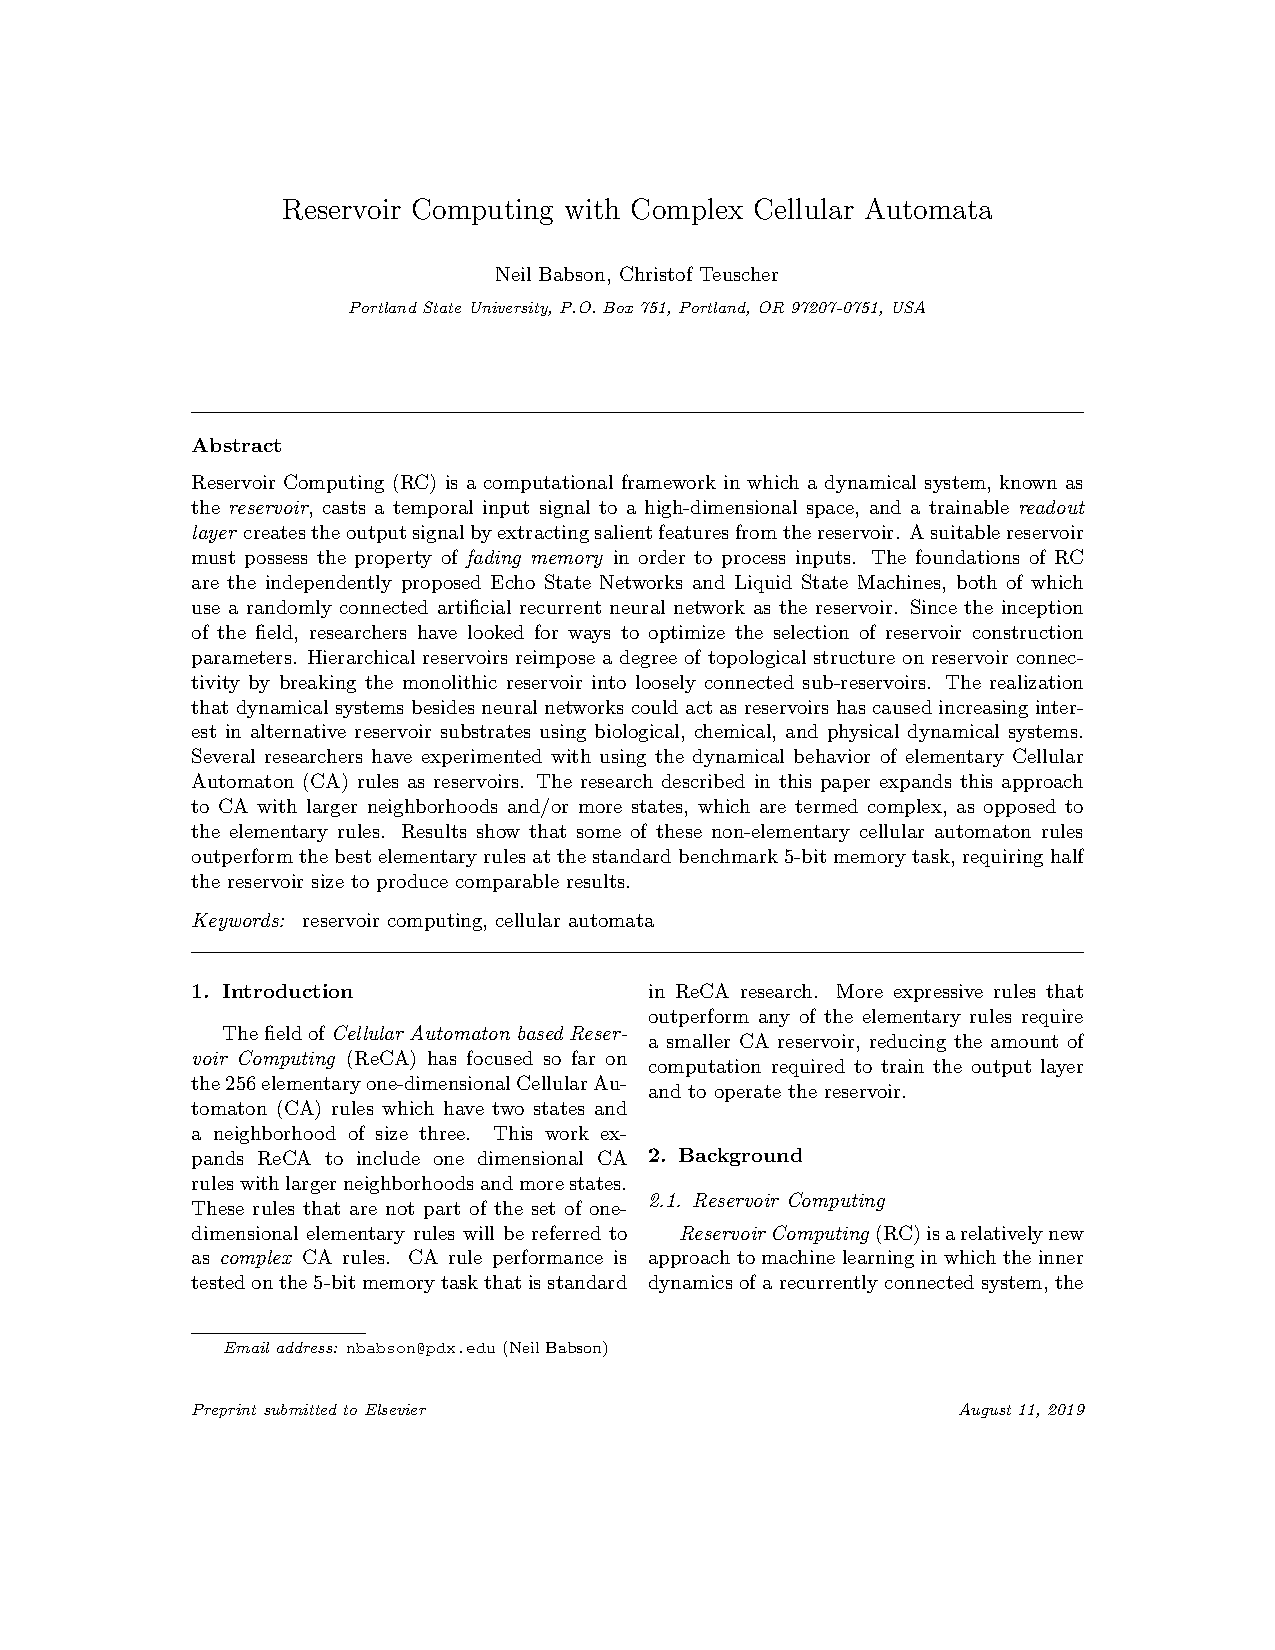
\includegraphics[width=0.5\textwidth]{CAReservoir.png}
    \caption{With a  Cellular Automata reservoir the input is mapped onto the 
        initial state of the CA and processed by repeated application of a 
            prespecified CA rule. \cite{yilmaz2015connectionist}}
            \label{CAReservoir}
            \end{figure}


     \begin{figure}[h!]
        \centering
            \includegraphics[width=1.0\textwidth]{DeepCA.png}
    \caption{ A hierarchical CA reservoir architecture.  The output from the 
        first CA reservoir is re-encoded and used as the input for a second 
            reservoir using a different CA rule. \cite{nichele2017deep}}

            \label{DeepCA}
            \end{figure}





     \subsection{Physical Reservoirs}
 %    \subsubsection{Water}
     C. Fernando and S. Sojakka took a very literal approach to implementing a 
     LSM, using a tank of water as the reservoir 
     \cite{fernando2003pattern}. The input was communicated to the reservoir by 
     motors driving weights up and down in the water, which translated the 
     input into a higher dimensional space of waves and ripples on the surface.  
     An output layer consisting of an array of perceptrons was trained on 
     images of the ripple patterns to solve the XOR problem and the speech 
     recognition task of differentiating the spoken words "zero" and "one".  
     Figure \ref{bucket} shows the experimental setup of the "liquid brain".  
     \par Several studies have used cultured neural cells stimulated by 
     microelectrode arrays, forming a hybrid biological-silicon computer 
     \cite{tanaka2018recent}. Figure \ref{neuron} shows the setup used by K.  
     Dockendorf et al. in which electrodes record the spiking activity of the 
     interconnected neurons in response to encoded voltage pulses. Another  
     biological reservoir made up of living organisms consisted of a population 
     of E.  Coli subjected to chemical inputs and temperature changes 
     \cite{jones2007there}. A readout layer of perceptrons generated the output 
     signal from measurement of protein levels in a sample of the E.  Coli.  
     \par  Recent research has explored a large number of other physical 
     reservoir implementations, demonstrating that various natural phenomena 
     possess information processing capability. Physical RC research areas 
     include spintronics, single-node time delayed circuits, optical node 
     arrays, and quantum systems \cite{tanaka2018recent}. Future work may lead 
     to the development of new information processing technologies based on RC 
     hardware. 


     \begin{figure}[h!]
        \centering
            \includegraphics[width=0.5\textwidth]{bucket.png}
    \caption{ A LSM in which the liquid is water.  Motors drive weights 
        creating input waves. An output layer of perceptrons is trained on wave 
            pattern images. \cite{fernando2003pattern}}
            \label{bucket}
            \end{figure}


     \begin{figure}[h!]
        \centering
            \includegraphics[width=0.5\textwidth]{neuron.png}
    \caption{ A network of cultured neurons stimulated by pulses of a 
        microelectrode array forms a hybrid biological-silicon computer.  
            Electrodes record the firing activity of the neural reservoir.  
            \cite{dockendorf2009liquid}}
	    \label{neuron}
            \end{figure}

%add to -- mention slow
\section{Conclusion}\label{conclusion}
In Reservoir Computing a high-dimensional dynamical system, the reservoir, 
   performs computational tasks.
This paper provides a brief overview of research on reservoir construction.  
Reservoir Computing has found success in a  number of temporal 
information-processing tasks. Since the inception of the Reservoir Computing 
paradigm with Echo State Networks in 2001 and Liquid State Machines in 2002, 
	 researchers have focused on ways to refine and optimize reservoir 
	 design. Recent work has shown that the internal dynamics of a variety 
	 of alternative substrates can be harnessed as reservoirs.  Reservoirs 
	 using physical systems could provide next-generation low-energy 
	 low-cost computational hardware, while biological reservoirs can shed 
	 light on information processing mechanisms in living brains.

\bibliographystyle{ieeetr}
\bibliography{CAReservoir}


\end{document}


